%%=============================================================================
%% Methodologie
%%=============================================================================

\chapter{\IfLanguageName{dutch}{Methodologie}{Methodology}}
\label{ch:methodologie}

%% TODO: Hoe ben je te werk gegaan? Verdeel je onderzoek in grote fasen, en
%% licht in elke fase toe welke stappen je gevolgd hebt. Verantwoord waarom je
%% op deze manier te werk gegaan bent. Je moet kunnen aantonen dat je de best
%% mogelijke manier toegepast hebt om een antwoord te vinden op de
%% onderzoeksvraag.

Na het literatuuronderzoek dat uitgeschreven is in de stand van zaken over wat \textit{elderspeak} en \textit{nursery tone} precies zijn, is het doel van deze bachelorproef om een website te ontwikkelen waarmee er \textit{elderspeak} kan gedetecteerd worden via een detector. In het literatuur werd er ook theoretisch beschreven wat AI is en welke types er zijn, wat en hoe \textit{natural language processing} werkt en hoe men achtergrond lawaai filtert.

Alle eigenschappen van \textit{elderspeak} worden herkend a.d.h.v. Python-bibliotheken en niet op basis van een zelf gemaakt AI-model. De reden hiervoor is dat men het warm water niet opnieuw moet uitvinden. Zo staafde \textcite{Beeckman2021} het volgende over zelf een AI-model te maken voor deze opstelling: ``Deze bachelorproef heeft geen meerwaarde kunnen aantonen voor het gebruik van een CNN. Wegens omstandigheden was het niet mogelijk te beschikken over een grote dataset wat leidt tot slechte voorspellingen van het model. Het model voorspelt een classificatie aan dezelfde accuraatheid dan dat gokken zou teweegbrengen. Dit maakt het huidige model onbruikbaar in de praktijk.''. Door deze bewering is de denkpiste in combinatie met de kleine dataset, die in dit onderzoek verzameld werd, over zelf een AI-model opstellen al snel van tafel geveegd. Ook de promotor Van Boven haalde aan dat er genoeg Python-bibliotheken ter beschikking waren om de opdracht op die manier tot een goed einde te brengen.

Sommige methoden konden gekopieerd worden van de bijlagen van de studenten die hiervoor aan gewerkt hebben, maar niet alle code stond beschreven in die bijlage. Daarnaast had \textcite{Standaert2021} geen GitHub-\textit{repository} waardoor de code niet snel kon hergebruikt worden. Ook zaten er af en toe kleine foutjes in de code waarbij het nodig was om die op te lossen. Daardoor zal er in Hoofdstuk~\ref{ch:vervolg} een deeltje aanbod komen over waarom het belangrijk is dat code gedeeld wordt.

\section{Berekeningen in \textit{back-end}}
Deze voorbeeldapplicatie, geschreven in Python en gebruikmakend van het \textit{micro-framework} Flask, is een webapplicatie die verschillende webpagina’s bevat. De code van de volledige Flask-applicatie is te vinden in bijlage~\ref{bijlage:flask}. Naast de inleidende pagina, zie schermafbeelding X, bevat deze ook een detector, zie schermafbeelding X, en een oplijsting van wat \textit{elderspeak} is, zie schermafbeelding X. Op die manier kunnen mensen, maar specifiek studenten in de zorg, actief en passief leren wat \textit{elderspeak} precies is. Enerzijds kunnen ze de eigenschappen te weten komen door zelf actief stukjes spraak op te nemen. Die wordt dan geanalyseerd zodat men kan zien welke eigenschappen er aanwezig waren. Anderzijds kunnen ze passief bekijken wat de eigenschappen zijn van \textit{elderspeak} en hoe men dat kan voorkomen.

De applicatie werd zo gemaakt waarbij men eerst twee jonge vrouwen ziet, een foto van HOGENT voor copyrightrechten, waarbij er gevraagd wordt om spraak in te spreken zoals men zou doen tegen hen. Dat geluid wordt dan geanalyseerd is voor de eigenschappen van toonhoogte en stemvolume. Daarna zal er een foto van een oudere vrouw getoond wordt in het rusthuis waarbij er gevraagd wordt om tegen haar te spreken. De twee parameters van daarvoor worden dan meegegeven zodat de correcte conclusies dan getrokken kunnen worden.

\subsection{\textit{Speech recognition}}
De basis van een groot deel van de applicatie is het herkennen van de spraak die wordt opgenomen op de website. Uiteraard moet dit niet van nul gemaakt worden, maar kan er gebruik gemaakt worden van een bestaande Python-bibliotheek. \textcite{Standaert2021} bestudeerde in zijn bachelorproef afgelopen jaar dat de beste optie is om de Google Speech Recognition-API te gebruiken omdat deze het beste presteert. Hij vatte dit samen in zijn conclusie: ``Uit verschillende onderzoeken of studies waar men verschillende ASR-systemen met elkaar vergeleken kwam de Google Speech-API er altijd als beste uit. En dit in alle aspecten.''. Daarnaast gebruikt de Google Speech-API ook \textit{natural language processing} of NLP om beter te kunnen weten wat er precies gezegd is geweest~\autocite{GoogleCloud2022}. Hoe dit precies in elkaar zit is te lezen in het literatuuronderzoek, namelijk in Hoofdstuk~\ref{ch:stand-van-zaken}.

Bij de spraakherkenning kwam er wel een groot probleem de kop op steken. De Google \textit{Speech Recognition}-API kon alleen overweg met \textit{wav}- en \textit{flac}-bestanden én kan maar een bepaalde periode, ongeveer 2 tot 3 minuten, gratis herkennen. Het probleem is dus dat de audio gecapteerd is in een \textit{mp3}-formaat. Hiervoor was het noodzakelijk om eerst een conversie te maken van \textit{mp3} naar \textit{flac} en om het audiobestand op te delen in deelbestandjes of \textit{chuncks}, zodat er geen betalende versie voor nodig was. De gebruikte technologie hierbij was ``ffmpeg''. Hoe de conversie precies gebeurt is te vinden tot in detail in bijlage~\ref{bijlage:speech_recognition}.

Het gebruiken van die API is relatief gemakkelijk. Een extra optie is dan ook ter beschikking om achtergrondlawaai een beetje weg te filteren. Door de optie `ajust\_for\_ambient\_noice(source)' aan te zetten, zal de bibliotheek zich wat aanpassen aan de geluidsbron zodat het beter de klanken kan horen alvorens die worden doorgestuurd naar de spraakherkenning-API. Deze methode gebruikt de techniek die beschreven is in het literatuuronderzoek over achtergrondlawaai.

Eens dit ingesteld is, worden de audiobestanden mee gegeven en krijgt het systeem de tekst terug waarvan het AI-model van Google de tekst herkend heeft. Uiteraard werkt dit niet feilloos, maar het is wel redelijk goed voor een gratis versie. Met deze grotere methode is de basis gelegd voor andere methoden die steunen op de tekst die herkend werd.

\subsection{Verkleinwoorden}
Voor de methode om verkleinwoorden te herkennen is er gefundeerd op de methode van \textcite{Standaert2021}. Daarbij wordt er gekeken of woorden langer zijn dan 3 letters en ze niet voorkomen in de lijst die geen verkleinwoorden zijn. Enkele voorbeelden die wel eindigen op ``-je'', ``-ke'', ``-kes'' of ``-jes'', maar voorbeelden die geen verkleinwoorden zijn, zijn: poffertje, meisje, koopje, etentje, dutje, toetje, mannelijke, vrouwelijke etc. De code voor deze methode kan gevonden worden in bijlage~\ref{bijlage:verkleinwoorden}.

\subsection{Herhalingen}
Om herhalingen te herkennen werd er evenals gebruikt gemaakt van de methode die \textcite{Standaert2021} geschreven had. Daarbij wordt er bijgehouden wat de vorige 25 woorden waren en bij herhalingen worden de woorden die herhaald worden bewaard in een lijst. Die zullen we later gebruiken om een mooie weergave te maken.
De code om herhalingen te detecteren is te vinden in bijlage~\ref{bijlage:herhalingen}.

\subsection{Collectieve voornaamwoorden}
Een voorbeeld van een collectief voornaamwoord is het gebruiken van: ``we'' / ``wij''. Om het voorbeeld te verduidelijken zijn de volgende zinnen gegeven: ``Gaan we onze patatjes opeten?'', ``Kunnen we alleen naar de wc?'', ``Awel, wat zijn we aan het doen?''.

Er wordt bijgehouden hoeveel keer er collectieve voornaamwoorden gebruikt worden in de tekst. Als een woord meer dan een keer voorkomt, dan beschouwt de applicatie dit dat het voorkomt. Dit is zo ingesteld omdat het niet mag worden weergegeven wanneer er iemand een keer het woord ``we'' gebruikt.
Wanneer er geen of minder dan twee collectieve voornaamwoorden gebruikt worden, zal de applicatie zeggen dat er geen of niet genoeg gebruikt werden.

Natuurlijk duiden twee of meer collectieve voornaamwoorden niet direct op \textit{elderspeak}, maar het geeft wel al een richting. De persoon in kwestie moet natuurlijk de theorie over \textit{elderspeak} weten en moet daarna ook kritisch zijn over het resultaat en dit kan via een zelfreflectie.

\subsection{Tussenwerpsels}
Het veelvuldig gebruik van tussenwerpsels is een eigenschap van \textit{elderspeak} en ook dit wordt herkend. Enkele voorbeelden van tussenwerpsels die herkend worden zijn: ``o'', ``oeps'', ``helaas'', ``hallo'', ``hey'', ``voila'' etc. De Google \textit{Speech Recognition}-API geeft soms verschillende varianten op het woord ``hey''. Zo worden de volgende vormen soms gegeven: ``hé'', ``hè'', ``he'', ``hey''. Om te voorkomen dat dat foute resultaten oplevert, worden al deze varianten herleid naar ``hey''.

De werkwijze om dit te detecteren is ongeveer dezelfde als bij de methode van de collectieve voornaamwoorden die te vinden is in bijlage~\ref{bijlage:tussenwerpsels}.

\subsection{Toonhoogte}
De toonhoogte is een bijzonder belangrijke eigenschap van \textit{elderspeak}. Deze eigenschap is ook volledig onafhankelijk van de gesproken tekst die herkend werd. Wanneer een persoon merkbaar hoger zal praten, zal de andere persoon direct voelen dat hij/zij behandeld wordt als een kind. Het is dan ook belangrijk dat deze functie goed werkt zodat de gebruikers direct weten wanneer ze (on)bewust hoger praten.

Deze methode werd al opgesteld door \textcite{Standaert2021} in zijn eindwerk van het vorige jaar. Wat hij berekende was de gemiddelde toonhoogte, uitgedrukt in Hz, van het gegeven audiobestand. Wat er aan deze applicatie toegevoegd is, is het berekenen of de toonhoogte hoger ligt bij de casus met de oudere vrouw dan de casus bij de twee jonger vrouwen.
Hoe dit gerealiseerd werd in de code is te vinden in bijlage~\ref{bijlage:toonhoogte}.

\subsection{Stemvolume}
De laatste eigenschap die geanalyseerd wordt in de applicatie is om te controleren of er luider gesproken wordt in het 2\textsuperscript{e} fragment dan in het 1\textsuperscript{ste}. Toch moet er hier een duidelijke kanttekening bij gemaakt worden. Wanneer een persoon bij de 2\textsuperscript{e} opname significant verder van de microfoon staat, zal de applicatie dit detecteren dat het niet luider zal zijn. Daarnaast moet er ook geweten zijn dat de meeste oudere mensen slechthorend zijn, waardoor men wel luider moet praten. Ondanks deze twee zaken vond ik het toch belangrijk om deze eigenschap te implementeren zodat men er wel eens bij stil staat dat niet iedereen slechthorend is of een hoorapparaat draagt.

Om een getal te verkrijgen dat het volume voorstelt, is er gebruik gemaakt van de pyln-bibliotheek die een BS.170 geluidsmeter aanmaakt in de code. Deze analyseert dan de audio en geeft een getal weer. Hoe dit precies geïmplementeerd werd is te vinden in bijlage~\ref{bijlage:stemvolume}.

\section{\textit{Front-end}}
\subsection{Geluid opnemen}
Het geluid opnemen gebeurt volledig aan de kant van de \textit{client} of de gebruiker. Wanneer er op de knop geduwd wordt om de audio-opname te starten, zullen er \textit{audiochunks } worden toegevoegd aan een lijst. Die worden na de opname allemaal samengevoegd tot een \textit{blob}, of een \textit{binary-large object}, die dan een \textit{mp3}-file aanmaakt.
Per casus wordt er ook een andere afbeelding en tekst getond boven de opneemknop.

\subsection{API-afhandeling}
Vanuit de front-end worden er \textit{API-requests} gestuurd met het audiobestand als bijlage naar de \textit{back-end}. De server analyseert dan de verschillende methodes. Wanneer alles onderzocht is, wordt alle data verzameld en via een JSON-formaat terug gestuurd naar de \textit{client}. Daar worden de resultaten ingevuld in de voorziene html-stukken.

\section{Testen}
Om een objectief beeld te kunnen verkrijgen hoe goed de applicatie werkt, zijn er automatische testen opgezet. De data die verzameld is via een online formulier, is te vinden op:  \url{https://www.jotform.com/form/213524968382060}. Deze werd in het begin van het twee semester verzameld. Eens de data opgeslagen was werd alle data beluisterd en handmatig gelabeld.

Nadien werd er een Python-script gemaakt die het testen van al die 54 bestanden automatiseerde. De audiobestanden die geklasseerd werden, waarbij er geen \textit{elderspeak} aanwezig bij was, werden gebruikt zoals in de echte webapplicatie om eerst een normaal stukje audio te hebben. Zo kan er toch vergelijken worden met een normale spraak en de spraak die erna komt. Nadien werden de geluidsopnames,  waarbij er wel \textit{elderspeak} bij aanwezig was, gebruikt voor het te testen van de applicatie zelf. De resultaten werden dan vergeleken met de gelabelde data.

Met deze resultaten konden er over de eigenschappen verkleinwoorden, hogere toonhoogte en hoger volume, een \texit{confusion matrix} gemaakt worden. Hierbij wordt er bepaald hoeveel correct negatieve, correct positieve, valse positieve en vals negatieve er aanwezig waren in het testset. Dit wordt dan in een matrix gegoten die visueel te vinden is in figuur~\ref{fig:confusion_matrix}. De resultaten daarvan zijn te vinden in het resultatenhoofdstuk, namelijk Hoofdstuk~\ref{ch:resultaten}.

\begin{figure}
    \centering
    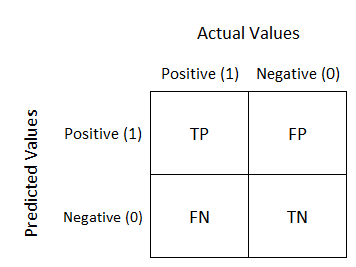
\includegraphics[width=0.6\textwidth]{./img/confusion_matrix}
    \caption{\label{fig:confusion_matrix} Confusion Matrix~\autocite{Jain2020}}
\end{figure}

\section{hosting?}
Om de applicatie te kunnen gebruiken tijdens (werkcolleges?) moet elke student toegang hebben tot de website. Hierdoor werd er bekeken hoe de software geïnstalleerd moest worden op een computer en hoe men de website beschikbaar maakt in het lokale netwerk.

TODO